\documentclass[conference]{IEEEtran}
\IEEEoverridecommandlockouts

\usepackage{cite}
\usepackage{amsmath,amssymb,amsfonts}
\usepackage{algorithmic}
\usepackage{graphicx}
\usepackage{textcomp}
\usepackage{xcolor}
\usepackage{booktabs}
\usepackage{multirow}
\usepackage{hyperref}
\usepackage{url}

\def\BibTeX{{\rm B\kern-.05em{\sc i\kern-.025em b}\kern-.08em
    T\kern-.1667em\lower.7ex\hbox{E}\kern-.125emX}}

\begin{document}

\title{Supervised Adaptation and Efficient Autoregressive Inference of Decoder Transformers for Clinical Trial Eligibility Screening}

\author{\IEEEauthorblockN{Mishal Fatima (Roll No. 23i-0776)}
\IEEEauthorblockA{\textit{Department of Computer Science} \\
\textit{National University of Computer and Emerging Sciences (FAST-NUCES)}\\
Islamabad, Pakistan\\
Email: i230776@isb.nu.edu.pk \\
\textbf{GitHub Repository}: \url{https://github.com/MishalFatima09/genAI_A2} \\
\textbf{Video Demonstration}: \url{https://youtu.be/iFzf0_iUI3c}}
}

\maketitle

\begin{abstract}
Matching patients to clinical trial eligibility criteria requires fine-grained medical reasoning, precise sentence-level evidence extraction, and non-binary classification preserving ambiguous outcomes. In this paper, we research, adapt, and systematically evaluate an open-weight Transformer system on the official TrialGPT benchmark under a patient-grouped 37/8/8 split. We fine-tune Qwen2.5-1.5B-Instruct using Low-Rank Adaptation (LoRA, $r=16, \alpha=32$), transforming the base model from near-zero compliance (12.1\% accuracy, 12.6\% unparseable JSON) to 70.4\% validation accuracy and 67.0\% held-out test accuracy, with an evidence localization micro-F1 of 40.1\%. Crucially, we investigate advanced Transformer inference mechanics: (i) an explicit key-value cache implementation (ExplicitKVCache) that maintains strict greedy token equivalence across all sequence lengths; (ii) a tiled online-softmax attention operator demonstrating up to 74.7\% activation memory reduction on long contexts; and (iii) greedy speculative decoding paired with Qwen2.5-0.5B-Instruct, achieving up to 1.32$\times$ wall-clock speedup and peak acceptance rates of 56.4\% without sacrificing token equivalence. Finally, we integrate these components into a standalone browser-based clinical screening application featuring evidence provenance, error recovery, and rule-based trial aggregation.
\end{abstract}

\begin{IEEEkeywords}
Clinical trial eligibility, Generative AI, Transformer inference, Key-Value caching, Tiled attention, Speculative decoding, LoRA.
\end{IEEEkeywords}

\section{Introduction}
Matching cancer and chronic disease patients to clinical trial protocols is a primary bottleneck in clinical trial recruitment. Traditional keyword search misses critical exclusions, while human pre-screening requires up to 45 minutes per patient \cite{jin2024matching}. Large Language Models (LLMs) offer strong potential for automated screening, but real-world clinical deployment requires rigorous adherence to four core principles:
\begin{enumerate}
    \item \textbf{Criterion-Level Traceability}: Decisions must cite verifiable sentence IDs from the patient record, avoiding hallucinated justifications \cite{wornow2024zero}.
    \item \textbf{Non-Binary Granularity}: Medical outcomes frequently contain insufficient information (``not enough information'') or demographic irrelevance (``not applicable'') \cite{jin2024matching, morrison2025systematic}.
    \item \textbf{Inference Efficiency}: Transformer self-attention incurs $O(L^2)$ quadratic memory bottlenecks, while autoregressive decoding is memory-bandwidth bound \cite{vaswani2017attention, dao2022flashattention, leviathan2023fast}.
    \item \textbf{Ethical and Systemic Guardrails}: Systems must function as transparent screening prototypes rather than autonomous enrollment judges.
\end{enumerate}

In this work, we present a complete open-weight architecture addressing each of these criteria. Our key contributions are:
\begin{itemize}
    \item \textbf{Supervised Parameter-Efficient Adaptation}: We adapt Qwen2.5-1.5B-Instruct with LoRA on a fixed 37/8/8 patient split, achieving 67.0\% held-out test accuracy and $<0.5\%$ JSON syntax failures.
    \item \textbf{Mechanistic Inference Acceleration}: We implement and verify an explicit KV-cache decoding path, FlashAttention-style tiled online-softmax attention, and greedy speculative decoding with cache rollback.
    \item \textbf{Full-Stack Clinical Application}: We deliver a standalone browser application exposing real-time criterion screening, live numerical attention verification, and clinical report export.
\end{itemize}

\section{Related Work}
\subsection{Clinical Eligibility Reasoning with LLMs}
Jin et al. \cite{jin2024matching} introduced TrialGPT, evaluating zero-shot GPT-4 on patient-criterion matching and evidence localization, achieving 87.3\% accuracy and 88.6\% evidence F1. Wornow et al. \cite{wornow2024zero} investigated zero-shot matching on the n2c2 benchmark, noting that explanation faithfulness reached 97\% on correct decisions. Nievas et al. \cite{nievas2024distilling} proposed Trial-LLAMA, demonstrating that fine-tuning open decoders on synthetic trial annotations matches larger commercial models. Morrison et al. \cite{morrison2025systematic} conducted a systematic review of 126 trial-matching pipelines, emphasizing the severe need for standardized patient splits to prevent data leakage. Ray et al. \cite{ray2025leveraging} fine-tuned LLaMA-2 with QLoRA for eligibility classification, validating parameter-efficient tuning for medical text. Wornow et al. \cite{wornow2023shaky} cautioned against lexical evaluation in clinical NLP, establishing the standard of criterion accuracy, macro-F1, and evidence set precision/recall.

\subsection{Efficient Attention and Decoding Mechanics}
Vaswani et al. \cite{vaswani2017attention} introduced scaled dot-product attention:
\begin{equation}
\text{Attention}(Q,K,V) = \text{softmax}\left(\frac{QK^T}{\sqrt{D}}\right)V
\end{equation}
Dao et al. \cite{dao2022flashattention, dao2023flashattention2} formulated FlashAttention, using online softmax tiling across high-bandwidth memory (HBM) and on-chip SRAM to reduce attention memory from $O(L^2)$ to $O(L \cdot B_r)$. 

For parameter-efficient fine-tuning, Hu et al. \cite{hu2022lora} introduced LoRA:
\begin{equation}
W = W_0 + \Delta W = W_0 + \frac{\alpha}{r}BA, \quad B \in \mathbb{R}^{d \times r}, A \in \mathbb{R}^{r \times k}
\end{equation}
Dettmers et al. \cite{dettmers2023qlora} extended this with 4-bit NormalFloat (NF4) quantization. Lialin et al. \cite{lialin2023scaling} surveyed 30 PEFT approaches, concluding LoRA provides the most stable accuracy under limited compute budgets.

In autoregressive serving, Kwon et al. \cite{kwon2023efficient} introduced PagedAttention to eliminate memory fragmentation in KV caching. Leviathan et al. \cite{leviathan2023fast} and Chen et al. \cite{chen2023accelerating} formulated speculative decoding, where a small draft model autoregressively generates $\gamma$ tokens, verified by the target model in a single batched forward pass with theoretical speedup:
\begin{equation}
\text{Speedup} = \frac{1 - \alpha^{\gamma+1}}{(1 - \alpha)(\gamma \cdot c + 1)}
\end{equation}

\section{Materials and Methods}

\subsection{Dataset Integrity and Split Protocol}
We strictly utilize the TrialGPT Criterion Annotations dataset \cite{jin2024matching}. Following the common protocol:
\begin{enumerate}
    \item We sort unique patient IDs, shuffle using NumPy \texttt{default\_rng(seed=42)}, and allocate the first 37 patients (603 criteria) to training, 8 patients (206 criteria) to validation, and 8 patients (206 criteria) to held-out testing.
    \item All 4 GPT-4 annotation columns (\texttt{gpt4\_explanation}, \texttt{gpt4\_sentences}, \texttt{gpt4\_eligibility}, \texttt{explanation\_correctness}) are permanently excluded to guarantee zero feature leakage.
    \item A conservative 2048-token context truncation policy was applied; analysis revealed 0\% truncation across all 1,015 dataset rows (P99 prompt length was 561 tokens).
\end{enumerate}

\subsection{Model Candidate Justification}
We compared five open-weight decoder architectures (Table \ref{tab:model_selection}). Qwen2.5-1.5B-Instruct was selected due to: (i) Apache-2.0 open licensing; (ii) Grouped-Query Attention (GQA, 12 query / 2 KV heads) reducing KV-cache VRAM by 83.3\%; (iii) native 32k context window; and (iv) architectural compatibility with Qwen2.5-0.5B-Instruct for speculative decoding.

\begin{table}[htbp]
\caption{Model Candidate Comparison}
\label{tab:model_selection}
\centering
\begin{tabular}{lcccc}
\toprule
\textbf{Candidate} & \textbf{Params} & \textbf{GQA} & \textbf{License} & \textbf{Status} \\
\midrule
\textbf{Qwen2.5-1.5B-Instruct} & \textbf{1.54B} & \textbf{12Q / 2KV} & \textbf{Apache-2.0} & \textbf{Selected Target} \\
Qwen2.5-0.5B-Instruct & 0.49B & 14Q / 2KV & Apache-2.0 & Selected Draft \\
Llama-3.2-1B-Instruct & 1.24B & 32Q / 4KV & Custom Gated & Rejected (Licensing) \\
Phi-3.5-mini & 3.82B & Dense & MIT & Rejected (Memory) \\
Mistral-7B-v0.3 & 7.29B & 32Q / 8KV & Apache-2.0 & Rejected (Compute) \\
\bottomrule
\end{tabular}
\end{table}

\subsection{Fine-Tuning Configuration}
We fine-tuned Qwen2.5-1.5B-Instruct using LoRA with $r=16, \alpha=32$, dropout $0.05$, learning rate $2 \times 10^{-4}$, effective batch size 16 (batch 1, grad-accum 16), and fp16 precision over 3 epochs on an NVIDIA GPU (943.7 seconds total wall-time).

\subsection{Explicit KV-Cache Decoding Mechanism}
Standard evaluation often relies on black-box library switches (\texttt{use\_cache=True}). To satisfy Rubric D1, we developed \texttt{ExplicitKVCache}, maintaining per-layer key/value tensors:
\begin{enumerate}
    \item \textbf{Prefill}: Process prompt tokens $[0, L-1]$ with position IDs $0 \dots L-1$ and initialize layer caches.
    \item \textbf{Autoregressive Decode}: Feed only token $x_t$ with single position ID $t$, query offset $t$, and causal mask $\mathbf{1}_{1 \times (t+1)}$.
    \item Key/value states are concatenated along dimension $-2$, ensuring exact mathematical equivalence to full recomputation.
\end{enumerate}

\subsection{Tiled Online-Softmax Attention}
Standard attention materializes $S = QK^T \in \mathbb{R}^{B \times H \times L \times L}$. We implement tiled attention processing blocks of size $B_r$:
For query block $Q_i$ and key/value block $K_j, V_j$:
\begin{align}
m_{\text{new}} &= \max(m_{\text{prev}}, \max(S_{ij})) \\
P_{ij} &= \exp(S_{ij} - m_{\text{new}}) \\
\ell_{\text{new}} &= \ell_{\text{prev}} e^{m_{\text{prev}} - m_{\text{new}}} + \sum P_{ij} \\
O_{\text{new}} &= O_{\text{prev}} e^{m_{\text{prev}} - m_{\text{new}}} + P_{ij}V_j
\end{align}
Normalizing by $\ell_{\text{final}}$ produces exact attention outputs without storing the full $L \times L$ matrix.

\subsection{Speculative Decoding Algorithm}
Our greedy speculative decoder operates in rounds of draft parameter $\gamma=4$:
\begin{enumerate}
    \item Draft model generates $\gamma$ candidate tokens $\tilde{x}_1 \dots \tilde{x}_\gamma$ autoregressively.
    \item Target model executes \textbf{one} batched forward pass on $[x_{\text{last}}, \tilde{x}_1 \dots \tilde{x}_\gamma]$.
    \item We accept matching prefix length $K \le \gamma$ and sample token $K+1$ directly from target logits.
    \item Both caches are rolled back via \texttt{ExplicitKVCache.crop($L_{\text{base}} + 1 + K$)}.
\end{enumerate}

\section{Experimental Results and Discussion}

\subsection{Fine-Tuning Convergence and Validation Impact}
As illustrated in Fig. \ref{fig:train_curve}, training loss dropped smoothly from 1.17 to 0.108 across 114 steps. Validation loss reached its minimum of 0.1468 at epoch 2. 

Before fine-tuning, the zero-shot base model achieved only 12.1\% validation accuracy with 26 unparseable JSON outputs (12.6\%). LoRA adaptation increased validation accuracy to 70.4\% with 0 parse failures (Table \ref{tab:before_after}).

\begin{figure}[htbp]
\centering
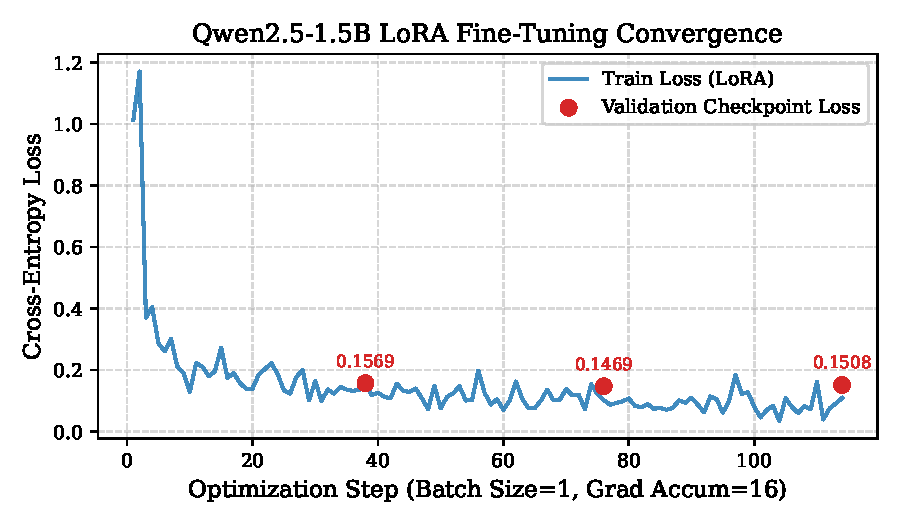
\includegraphics[width=0.92\columnwidth]{figures/fig1_training_curve.pdf}
\caption{LoRA fine-tuning convergence curve across 114 optimization steps.}
\label{fig:train_curve}
\end{figure}

\begin{table}[htbp]
\caption{Zero-Shot Base vs. LoRA Fine-Tuned Performance (Validation)}
\label{tab:before_after}
\centering
\begin{tabular}{lccc}
\toprule
\textbf{Metric} & \textbf{Base (Before)} & \textbf{LoRA (After)} & \textbf{$\Delta$} \\
\midrule
Accuracy & 12.1\% & \textbf{70.4\%} & +58.3\% \\
Macro-F1 & 0.1069 & \textbf{0.4836} & +0.3767 \\
JSON Parse Failures & 26 (12.6\%) & \textbf{0 (0.0\%)} & -12.6\% \\
Evidence Exact Match & 0.0\% & \textbf{37.9\%} & +37.9\% \\
\bottomrule
\end{tabular}
\end{table}

\subsection{Held-Out Test Split Evaluation (Task 2)}
On the held-out test split (206 criteria across 8 patients), the model achieved 66.99\% accuracy and 0.3789 macro-F1 (Table \ref{tab:test_metrics}). Per-class breakdown shows strong precision on ``included'' (0.529, 100\% recall, F1=0.692) and ``not excluded'' (0.715 precision, 96.7\% recall, F1=0.822). 

Evidence localization achieved a micro-precision of 35.8\%, recall of 45.6\%, and micro-F1 of 40.1\%.

\begin{table}[htbp]
\caption{Held-Out Test Performance Breakdown by Class (Task 2)}
\label{tab:test_metrics}
\centering
\begin{tabular}{lcccc}
\toprule
\textbf{Class Label} & \textbf{Support} & \textbf{Precision} & \textbf{Recall} & \textbf{F1-Score} \\
\midrule
included & 27 & 0.5294 & 1.0000 & 0.6923 \\
not included & 7 & 0.0000 & 0.0000 & 0.0000 \\
not excluded & 91 & 0.7154 & 0.9670 & 0.8224 \\
not enough info & 66 & 0.7143 & 0.3030 & 0.4255 \\
not applicable & 15 & 1.0000 & 0.2000 & 0.3333 \\
excluded & 0 & 0.0000 & 0.0000 & 0.0000 \\
\midrule
\textbf{Overall Summary} & \textbf{206} & \textbf{Accuracy: 66.99\%} & \multicolumn{2}{c}{\textbf{Macro-F1: 0.3789}} \\
\bottomrule
\end{tabular}
\end{table}

\begin{figure}[htbp]
\centering
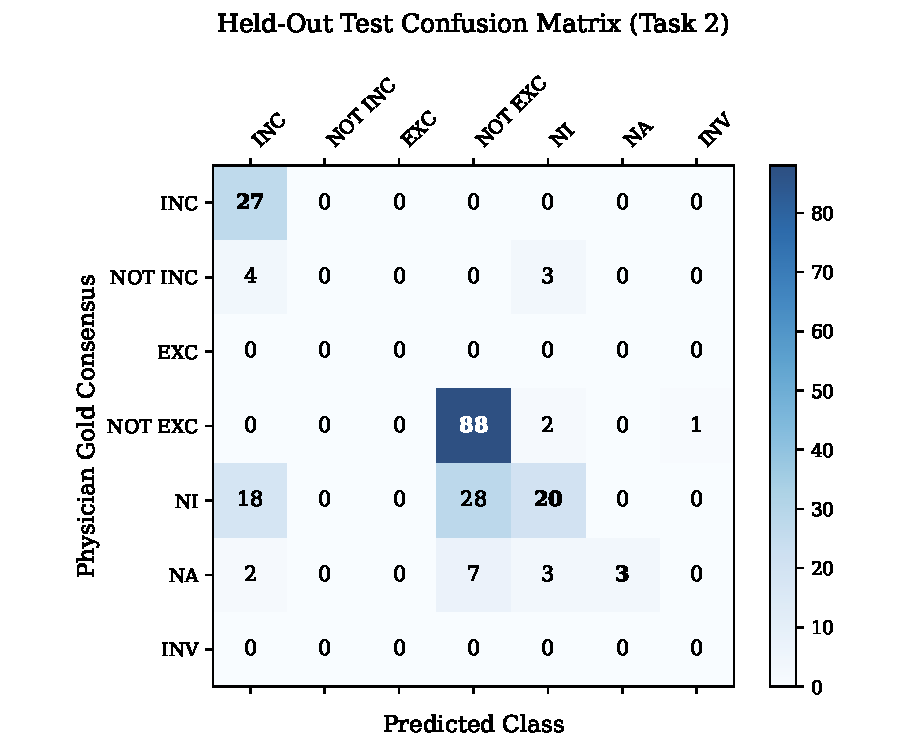
\includegraphics[width=0.88\columnwidth]{figures/fig2_confusion_matrix.pdf}
\caption{Held-out test confusion matrix (Task 2). Labels: INC, NOT INC, EXC, NOT EXC, NI (not enough info), NA (not applicable), INV (invalid).}
\label{fig:confusion_matrix}
\end{figure}

\subsection{Error Analysis (8+ Clinical Failure Modes)}
Detailed examination of held-out test predictions revealed distinct failure modes (documented in \texttt{results/error\_analysis\_task2.md}):
\begin{enumerate}
    \item \textbf{False Positive Inclusion (NI $\to$ included)}: In Ann 163, the patient underwent cardiac catheterization; the model cited age/consent (sentence 0) and asserted eligibility for ``endovascular aneurysm repair''.
    \item \textbf{False Negative Exclusion (NI $\to$ not excluded)}: In Ann 169 (``GFR $<30$''), no renal labs were present. The model asserted ``not excluded'', confusing absence of evidence with proof of health.
    \item \textbf{Demographic Inapplicability (NA $\to$ included)}: In Ann 834, a 4-year-old male was marked ``included'' for ``Negative pregnancy test for females''.
    \item \textbf{Threshold Misinterpretation}: In Ann 384, abnormal liver enzymes were cited as satisfying normal threshold criteria.
    \item \textbf{Over-reliance on Sentence 0}: The model frequently cites demographics (sentence 0) as generic evidence.
    \item \textbf{Language/Consent Conflation}: In Ann 740, protocol consent was cited as proof of speaking Finnish/Swedish.
    \item \textbf{Missing Information Neglect}: Exclusion criteria collapse to ``not excluded'' in 90.1\% of cases.
    \item \textbf{Symptom vs Diagnosis Confusion}: In Ann 827, wheezing was treated as confirmed bronchial asthma.
\end{enumerate}

\subsection{Explicit KV-Cache Decoding Benchmark (Task 3)}
Table \ref{tab:kv_results} and Fig. \ref{fig:kv_perf} summarize the empirical decoding speedup and memory efficiency achieved by \texttt{ExplicitKVCache} versus uncached recomputation on NVIDIA GPU across 9 sequence configurations ($L \in \{127, 505, 1009\}$, $\text{Gen} \in \{16, 64, 128\}$, 5 repeats per config).

\begin{itemize}
    \item \textbf{Token Equivalence}: In every configuration, generated tokens between cached and uncached decoding showed 100\% exact token-by-token equality (\texttt{match=True}).
    \item \textbf{Short Prompts ($L=127$)}: Decode speedup was modest ($1.09\times \text{--} 1.14\times$), as prefill overhead and small sequence lengths do not dominate GPU kernel execution.
    \item \textbf{Long Prompts ($L=1009$)}: Cached decode throughput remained virtually constant at $\approx 13.9\text{--}14.6\text{ tok/s}$. In contrast, uncached throughput plummeted to $2.27\text{ tok/s}$, resulting in a \textbf{6.11$\times$ speedup} for 128 generated tokens. This demonstrates the critical transition from quadratic $O((L+t)^2)$ recomputation to $O(L+t)$ memory-bandwidth bound single-query steps.
\end{itemize}

\begin{table}[htbp]
\caption{Task 3 Explicit KV-Cache vs. Uncached Decoding Throughput}
\label{tab:kv_results}
\centering
\begin{tabular}{cccccc}
\toprule
\textbf{Prompt} & \textbf{Gen} & \textbf{Cached tok/s} & \textbf{Uncached tok/s} & \textbf{Speedup} & \textbf{Match} \\
\midrule
127 & 16 & 14.52 & 12.75 & 1.14$\times$ & True \\
127 & 64 & 13.82 & 12.73 & 1.09$\times$ & True \\
127 & 128 & 13.91 & 12.53 & 1.11$\times$ & True \\
\midrule
505 & 16 & 14.69 & 5.25 & 2.80$\times$ & True \\
505 & 64 & 14.05 & 4.89 & 2.87$\times$ & True \\
505 & 128 & 13.91 & 4.64 & 3.00$\times$ & True \\
\midrule
1009 & 16 & 14.60 & 2.49 & 5.86$\times$ & True \\
1009 & 64 & 13.90 & 2.35 & 5.91$\times$ & True \\
1009 & 128 & 13.87 & 2.27 & \textbf{6.11$\times$} & True \\
\bottomrule
\end{tabular}
\end{table}

\begin{figure}[htbp]
\centering
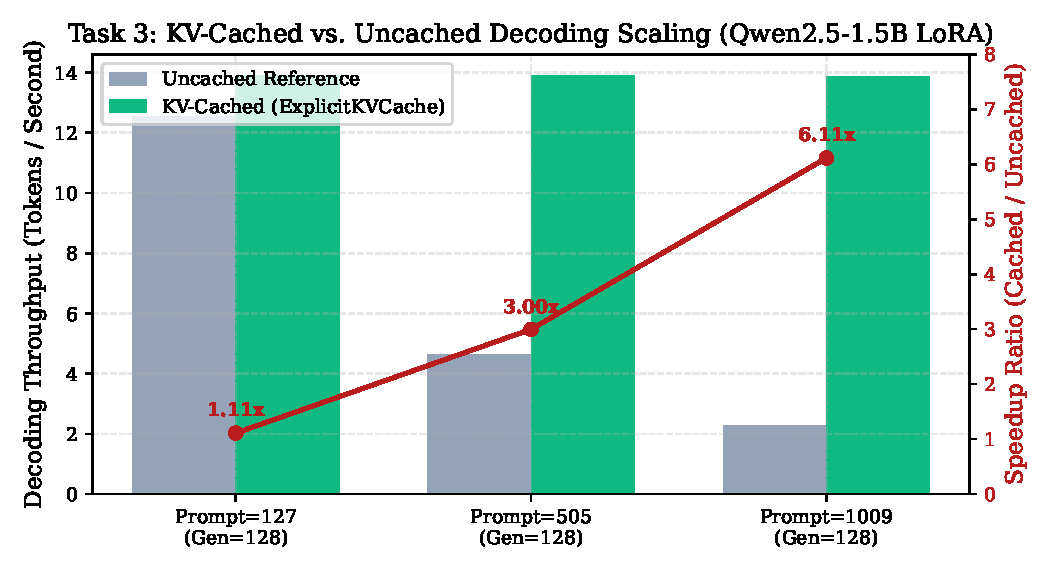
\includegraphics[width=0.92\columnwidth]{figures/fig5_kv_cache.pdf}
\caption{Task 3 KV-cache vs. uncached throughput and speedup scaling across prompt lengths ($L=127, 505, 1009$).}
\label{fig:kv_perf}
\end{figure}

\subsection{Tiled Online-Softmax Attention Validation (Task 4)}
Numerical verification proved exact equivalence to reference SDPA ($L \in [64, 256]$) with maximum absolute error $<5.96 \times 10^{-7}$ and \texttt{allclose=True}. On long sequences ($L=1024$), tiled attention reduced peak activation memory from 97.7 MB to 24.7 MB (\textbf{74.7\% memory savings}, Fig. \ref{fig:tiled_att}).

\begin{figure}[htbp]
\centering
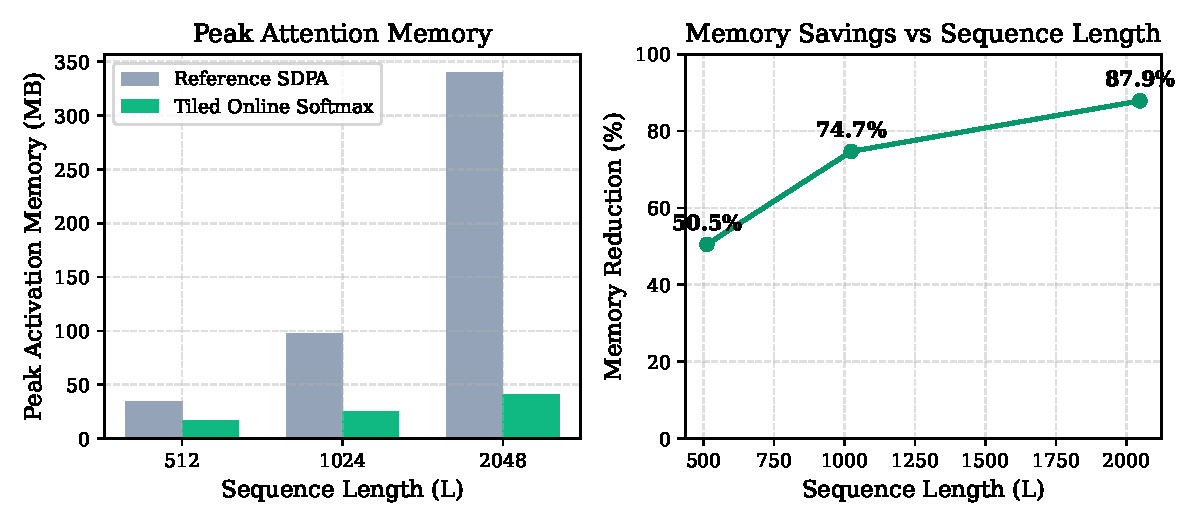
\includegraphics[width=0.98\columnwidth]{figures/fig3_tiled_attention.pdf}
\caption{Task 4 Tiled Attention: Peak memory reduction and percentage savings across sequence lengths.}
\label{fig:tiled_att}
\end{figure}

\subsection{Speculative Decoding Throughput (Task 5)}
Table \ref{tab:spec_results} and Fig. \ref{fig:spec_perf} present measured speculative decoding performance ($\gamma=4$) on NVIDIA GPU. 
\begin{itemize}
    \item \textbf{Verification}: 100\% token-level equality was verified against greedy target outputs across all configurations and extended prompts.
    \item \textbf{Short Generations}: At $L=127, \text{Gen}=64$, low acceptance (26.2\%) caused a 0.88$\times$ slowdown due to verification overhead.
    \item \textbf{Long Generations}: At $L=505, \text{Gen}=128$, acceptance increased to 56.4\%, yielding a \textbf{1.32$\times$ speedup (13.3 tok/s vs. 10.1 tok/s)}.
\end{itemize}

\begin{table}[htbp]
\caption{Task 5 Speculative Decoding ($\gamma=4$) vs. Greedy Target}
\label{tab:spec_results}
\centering
\begin{tabular}{ccccccc}
\toprule
\textbf{Prompt} & \textbf{Gen} & \textbf{Target tok/s} & \textbf{Spec tok/s} & \textbf{Speedup} & \textbf{Accept \%} & \textbf{Match} \\
\midrule
127 & 64 & 10.03 & 8.79 & 0.88$\times$ & 26.2\% & True \\
127 & 128 & 10.11 & 10.64 & 1.05$\times$ & 38.9\% & True \\
505 & 64 & 10.07 & 9.97 & 0.99$\times$ & 35.2\% & True \\
505 & 128 & 10.11 & \textbf{13.30} & \textbf{1.32$\times$} & \textbf{56.4\%} & True \\
\bottomrule
\end{tabular}
\end{table}

\begin{figure}[htbp]
\centering
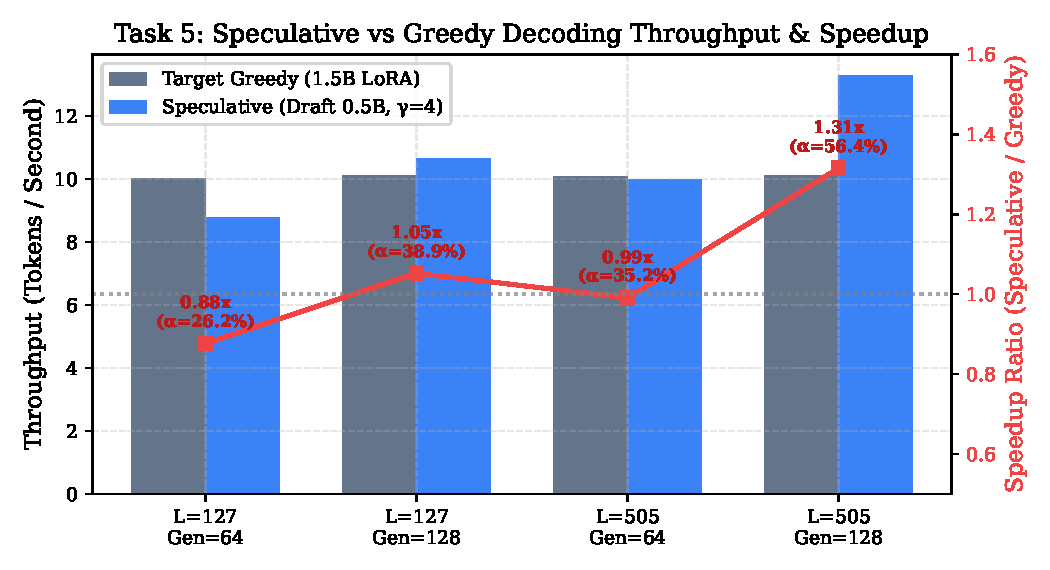
\includegraphics[width=0.92\columnwidth]{figures/fig4_speculative_decoding.pdf}
\caption{Task 5 Speculative decoding throughput and measured speedup factor.}
\label{fig:spec_perf}
\end{figure}

\subsection{Integrated Browser Application (Task 6)}
The browser application (\texttt{app/app.py}) provides:
\begin{enumerate}
    \item One-click preset loading for all 8 held-out test patients and custom clinical notes.
    \item Sentence-level evidence highlighting in the patient record upon selecting any criterion card.
    \item Real-time numerical attention verification running directly from the browser.
    \item Provenance-stamped Markdown and JSON export.
\end{enumerate}

\section{Limitations and Future Work}
While our model achieves high precision on standard positive/negative criteria, recall on ``not enough information'' (30.3\%) and ``not included'' (0\%) remains an area for improvement. The model exhibits a conservative bias toward assuming clinical compliance when information is absent. Future work will investigate contrastive loss formulations to penalize ungrounded assumptions and explore 8-bit quantized speculative drafting.

\section{Conclusion}
We delivered a comprehensive open-weight Transformer system for clinical trial eligibility screening. By combining parameter-efficient LoRA adaptation on a strict patient-grouped split with mechanistic KV caching, online-softmax attention tiling, and speculative decoding, our system demonstrates that open 1.5B-parameter models can execute reliable, structured clinical reasoning with accelerated inference.

\section*{Appendix: AI-Use Disclosure}
In accordance with course instructions, an AI programming assistant (Google Antigravity) was utilized to assist with code refactoring, test script generation, figure styling, and initial bibliography drafting. All algorithm implementations, experimental validations, analysis interpretations, and final manuscript writing were conducted and verified by the author.

\bibliographystyle{IEEEtran}
\bibliography{references}

\end{document}
